\chapter{开发$H\to WW$质量去相关多分类标记器}
\label{chap5}
\fontsize{12bp}{14.4pt}
我们基于上一章的ParticleNet网络架构,通过修改网络输入输出,产生专用训练样本,并结合质量去相关技术,开发了CMS实验中首个针对大动量$H\to WW$的质量去相关版本多分类标记器。

\section{质量去相关技术}
对于质量相关版本的标记器,神经网络会学习到信号样本与本底样本质量分布的差异,并且把它作为区分信号与本底的潜在判别条件,对于这样训练出来的标记器,在把本底事件误鉴别为信号事件时,会更倾向于挑选出质量分布接近信号样本的本底事件,从而对于数据中通过标记器的本底事件,在质量谱上会形成信号峰下的峰状本底,这种情况也叫做质量雕刻(mass-sculpting)。这显然对于我们从质量谱中提取信号造成了不小的困难,因此质量去相关的标记器就显得尤为重要。

\begin{figure}[H]
 \centering
 \caption{质量关联标记器对QCD本底的质量雕刻现象(与质量去相关标记器的对比)\cite{jet-tagging-algorithms}}
 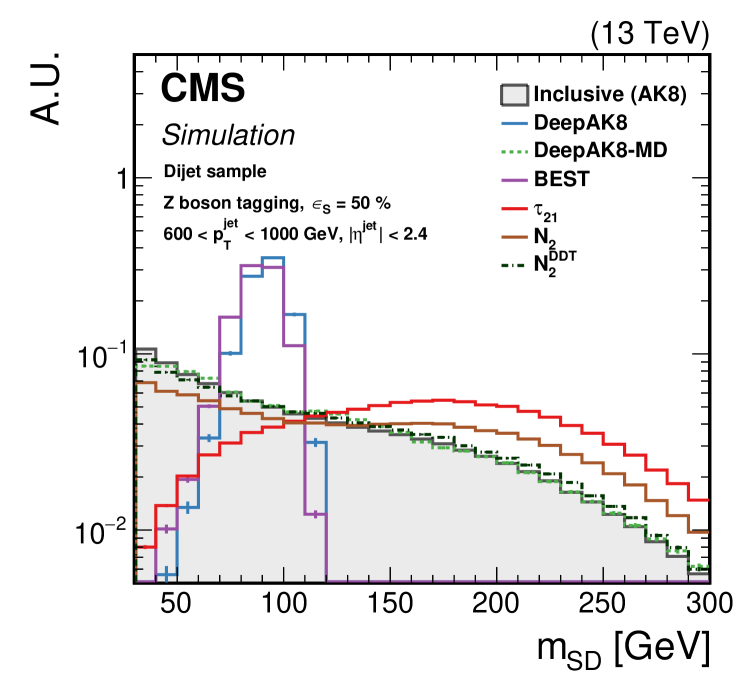
\includegraphics[height=10cm, width=11cm]{pictures/nonMDtagger.png}
 \label{fig:5.1}
\end{figure}

从以上信息我们知道,当训练中的信号和本底样本有明显不同的质量分布时,训练出来的标记器在推理筛选本底样本时就会出现质量雕刻的现象。所以,如果训练样本的信号和本底的质量分布一致,标记器则不会学习到二者的质量信息作为区分条件,从而不会在推理筛选本底样本时出现质量雕刻现象\cite{deepak8andmass-decorrelation}。

要实现这点,最简单直接的办法就是在训练时对信号和本底的分布进行重新加权,但是这往往还有其他隐患,例如:
\begin{enumerate}[(1)]
    \item 如果信号样本的质量分布峰过于集中,也就是说,在信号质量窗外的事例统计量过低,这样对信号重加权时,会导致信号窗内的高峰被极大压低到和信号窗外事件相同的高度,从而造成大量真实信号没有被选中参与训练,是一种极大的浪费和欠拟合的隐患。
    \item 同时,对于远离信号窗的事例,也很难被重建出来,进一步加大了训练和推理的难度。
\end{enumerate}

综合以上两点原因,最好的做法就是尽可能使用于训练的信号样本的质量分布尽可能平滑(避免极端事例的低统计量过度压低加权),信号窗尽可能大(避免远离信号窗事例难以重建)。所以我们的做法是:设计带有一维$ m_{SD}$平分布的专用MC样本以供训练,可以通过产生并合并不同共振态质量的样本实现。(例如,产生变质量$m_X$的$X\to bb$,$X\to cc$,$X\to qq$样本以训练通用二分叉喷注标记)

\section{分类标签}
因为我们采用的ParticleNet神经网络属于监督学习范畴,所以对于训练样本,我们在产生的同时还要给它们贴上正确的标签,才能使得网络学到如何区分不同标签的喷注。

对于训练样本的喷注标记,我们使用了一套专门设计的代码\cite{dnntuples}以产生样本和打上训练标签,在训练样本的粒子层级,利用粒子的产生信息,给粒子组成的喷注打上适当的标签,同时要求打上标签的喷注都满足$\Delta R=0.8$以产生AK8喷注。该产生代码的喷注标签部分见\textbf{附录\ref{appendix:labeling}}。

\subsection{信号分类标签}
对于我们关心的$H\to WW\to anything$的信号,我们主要关心两种衰变场景:一种是两个W都进行强子化衰变,也称作全强子衰变;另一种是一个W进行强子化衰变一个W进行轻子化衰变,也被称作半轻衰变)。所以,我们采用了以下的末态分类标签:
\begin{itemize}
    \item $\mathbf{4q}$:$H\to W(2q)W(2q)$,并且重建出4分叉的AK8喷注
    \item $\mathbf{3q}$:$H\to W(2q)W(2q)$,但仅重建出3分叉的AK8喷注
    \item $\mathbf{e\nu_e qq}$:$H\to W(e\nu_e)W(2q)$喷注
    \item $\mathbf{\mu\nu_\mu qq}$:$H\to W(\mu\nu_\mu)W(2q)$喷注
    \item $\mathbf{\tau_e\nu_eqq}$:$H\to W(\tau\nu)W(2q)$,$\tau$接着衰变为电子等产物
    \item $\bm{\tau_\mu\nu qq}$:$H\to W(\tau\nu)W(2q)$,$\tau$接着衰变为$\mu$子等产物
    \item $\mathbf{\tau_h\nu qq}$:$H\to W(\tau\nu)W(2q)$,$\tau$接着进行强子化衰变
\end{itemize}
\subsection{本底分类标签}
对于我们关注的QCD本底喷注,我们可以按喷注中的子喷注结构对其进行分类如下:
\begin{itemize}\label{eq:5.2}
    \item \textbf{QCD(bb)}:QCD喷注中有两个b夸克子喷注
    \item \textbf{QCD(cc)}:QCD喷注中有两个c夸克子喷注
    \item \textbf{QCD(b)}:QCD喷注中有一个b夸克子喷注
    \item \textbf{QCD(c)}:QCD喷注中有一个c夸克子喷注
    \item \textbf{QCD(others)}:具有其他子结构的QCD喷注
\end{itemize}

\section{数据集}
\subsection{训练集和验证集}
我们产生了专门设计的私人HWW信号样本和基于官方设置产生的QCD本底样本,同时按照15:1的比例把它们分成训练集和验证集供训练使用。
\subsubsection{信号样本}
因为我们的目标是开发一个质量去相关的标记器,所以我们的信号MC样本有以下特点:
\begin{itemize}
    \item 样本基于2017 ultra-legacy,总共有两千五百多万事例。
    \item 使用变质量X的$X\to WW$衰变样本,设置的产生级别质量分布区间为$15 [\si{GeV}]\leq m_X\leq 250[\si{GeV}]$,并保证合并起来的总信号样本具有平坦的产生级别质量分布,同时设置W质量为$m_W=80[\si{GeV}]$。
    \item 使用JHUGen产生子实现$X\to WW\to4q/\ell \nu qq$衰变以更好模拟衰变产物的自旋关联。
    \item 喷注通过$\Delta R=0.8$的事实匹配以满足AK8喷注的要求。
    \item 喷注通过粒子级别的事实匹配打上$4q,\ 3q,\ e\nu qq,\ \mu\nu qq,\ \tau_e\nu qq,\ \tau_\mu\nu qq,\ \tau_h\nu qq$七个标签之一。
\end{itemize}

\subsubsection{本底样本}
QCD本底样本有以下几个特点:
\begin{itemize}
    \item 样本基于2017 ultra-legacy,总共有两千八百多万事例。
    \item 喷注通过$\Delta R=0.8$的事实匹配以满足AK8喷注的要求。
    \item 喷注通过粒子级别的事实匹配打上QCD(bb,cc,b,c,others)五个标签之一。
\end{itemize}
\subsection{测试集}
测试集以训练集和验证集相同的方式产生。对于测试集中的信号样本,Higgs的产生级别质量固定在标准模型125[GeV]处(训练集中不包含这个质量点产生的样本),包含约四十万个事例。对于测试集中的QCD本底样本,以和训练集相同的方式产生,共有约五百万左右事例。


\section{标注器设置}
\subsection{预挑选条件}
我们要求进入标注器的事例满足以下条件:
\begin{itemize}
    \item 每个事例仅由一个喷注构成,并且这个喷注通过了Pile-up的紧挑选条件
    \item 喷注的横向动量满足$200[\si{GeV}]<p_T<2500[\si{GeV}]$
    \item 喷注的soft-drop质量满足$20[\si{GeV}]\leq m_{SD}<260[\si{GeV}]$
    \item 对于训练样本,喷注要通过粒子级别的事实匹配满足12个标签分类之一
\end{itemize}
以此保证我们设计的标记器是针对大动量$H\to WW$场景,并且以此通过预筛选去掉大量的无关本底,从而提高标记器的鉴别能力并降低训练速度。

\subsection{重加权设置}
训练用的信号样本和本底样本合起来共有12个分类标签,我们要产生质量去相关的标记器,就得对用于训练的信号和本底进行质量和横向动量的二维分区间重加权。

\textbf{重加权的定义}是:对于某个被重加权的标签分类,指定分布上的每个区间都要持有相同数量的事例数,并且来自每个分类的事例数占比要符合我们预定义的分类权重

现在我们要对信号和QCD本底样本同时在$[p_T,m_{SD}]$二维分布上做重加权操作,对soft-drop质量$m_{SD}$的分bin区间为从20[GeV]到260[GeV]每隔10[GeV]分一个bin,对横向动量$p_T$的分bin区间为[200, 251, 316, 398, 501, 630, 793, 997, 1255, 1579, 1987, 2500],单位为[GeV]。(值得注意的是,对$p_T$分bin按照对数等bin宽的选择,这是因为有对QCD的$p_T$分布呈指数衰减的经验分布,所以采用对数等bin宽可以尽可能使得分bin后直方图高度均匀)

定义各个分类标签定义的重加权权重时,我们把\eqref{eq:5.2}中的五个QCD子分类都合并成$QCD$标签分类参与加权。最后得到分类权重的如下:
\begin{equation}
\begin{split}
    4q:3q:e\nu qq:\mu\nu qq:\tau_e\nu qq:\tau_\mu\nu qq:\tau_h\nu qq:QCD \\
    =0.34:0.08:0.2:0.2:0.03:0.03:0.12:1 &
\end{split}
\end{equation}
这里各个信号子分类的权重经过我们精心挑选,使得每个权重与该分类在信号中的占比接近,从而提高训练速度。

\subsection{神经网络输入}
我们针对粒子候选者(ParticleFlow candidates)和重建出的次级顶点两类对象,定义如下变量作为标记器神经网络的输入,如下\textbf{表\ref{table:5.1}}所示。
\begin{table}[htbp]
    \caption{神经网络输入\cite{Javier}}\label{table:5.1}
    \centering
    \begin{tabular}{>{\centering\arraybackslash}p{2.5cm}%
    >{\centering\arraybackslash}p{3cm}%
    >{\centering\arraybackslash}p{9cm}}
    \toprule\toprule
    \textbf{对象} & \textbf{变量} & \textbf{描述}\\
    \midrule
    \multirow{25}{*}{粒子候选者} & $\eta_{rel}$ & 相对于AK8喷注主轴的赝快度$\Delta \eta$\\
    & $\phi_{rel}$ & 相对于AK8喷注主轴的方位角$\Delta \phi$\\
    & $\log{p_T}$ & $p_T$的对数\\
    & $\log{E}$ & 能量的对数\\
    & $|\eta|$ & 赝快度的绝对值\\
    & charge & 电荷\\
    & isEl & 是否被鉴别为电子\\
    & isMu & 是否被鉴别为$\mu$子\\
    & isGamma & 是否被鉴别为光子\\
    & icChargedHad & 是否被鉴别为带电强子\\
    & isNeutralHad & 是否被鉴别为中性强子\\
    & VTX\_ass & 初级顶点的关联品质\\
    & lostInnerHits & 内部硅径迹器的击中数信息\\
    & normchi2 & 径迹拟合的归一化$\chi^2$\\
    & quality & 径迹品质\\
    & dz & 纵向冲击参数:在z方向到初级顶点的最近距离\\
    & dzsig & 纵向冲击参数显著度\\
    & dxy & 横向冲击参数:在横切面到束流的最近距离\\
    & dxysig & 横向冲击参数显著度\\
    & BTag\ $\eta_{rel}$ & 径迹相对AK8喷注主轴的赝快度$\Delta \eta$\\
    & BTag\ $p_T$ ratio & 径迹垂直AK8喷注主轴的分动量与合动量之比\\
    & BTag $p_{\parallel}$ Ratio & 径迹平行AK8喷注主轴的分动量与合动量之比\\
    & BTag Sip3dVal & 径迹的三维正负冲击参数\\
    & BTag Sip3dSig & 径迹的三维正负冲击参数显著度\\
    & BTag JetDistVal & 径迹到AK8喷注主轴的最小接近距离\\
    \midrule
    \multirow{11}{*}{次级顶点} & $\eta_{rel}$ & 相对于AK8喷注主轴的赝快度$\Delta \eta$\\
    & $\phi_{rel}$ & 相对于AK8喷注主轴的方位角$\Delta \phi$\\
    & $m_{SV}$ & 次级顶点不变质量\\
    & $\log{p_T}$ & $p_T$的对数\\
    & $|\eta|$ & 赝快度的绝对值\\
    & $N_{track}$ & 径迹条数\\
    & normchi2 & 顶点拟合的$\chi^2$除以自由度\\
    & dxy & 横向飞行距离\\
    & dxysig & 横向飞行距离显著度\\
    & d3d & 三维飞行距离\\
    & d3dsig & 三维飞行距离显著度\\
    \bottomrule\bottomrule
\end{tabular}
\end{table}

\subsection{神经网络输出}
我们的标记器(深度神经网络)的输出为给每个喷注打上的以下12个不同分类的分数,分数越高代表越有可能属于这个类
\begin{equation*}
    \textbf{SCORE}:\ \left\{
    \begin{aligned}
    HWW&(4q)\\
    HWW&(3q)\\
    HWW&(e\nu qq)\\
    HWW&(\mu\nu qq)\\
    HWW&(\tau_e\nu qq)\\
    HWW&(\tau_\mu\nu qq)\\
    HWW&(\tau_h\nu qq)\\
    QCD&(bb)\\
    QCD&(cc)\\
    QCD&(b)\\
    QCD&(c)\\
    QCD&(others)\\
    \end{aligned}
    \right.
\end{equation*}

然后对于某个信号道vs.QCD本底的标记任务,我们可以定义判别分数为:
\begin{equation}
    discriminant\_score\equiv\frac{score\_signal}{score\_signal + score\_QCD}
\end{equation}
\section{标记器在测试集上效果}
同时对信号样本标记与本底样本标记的ROC图如下,其纵轴是QCD被误标记信号的效率,横轴是信号被标记的效率
\begin{figure}[H]\label{fig:5.2}
 \centering
 \caption{标记器的$H\to WW\to 4q$标记效果}
 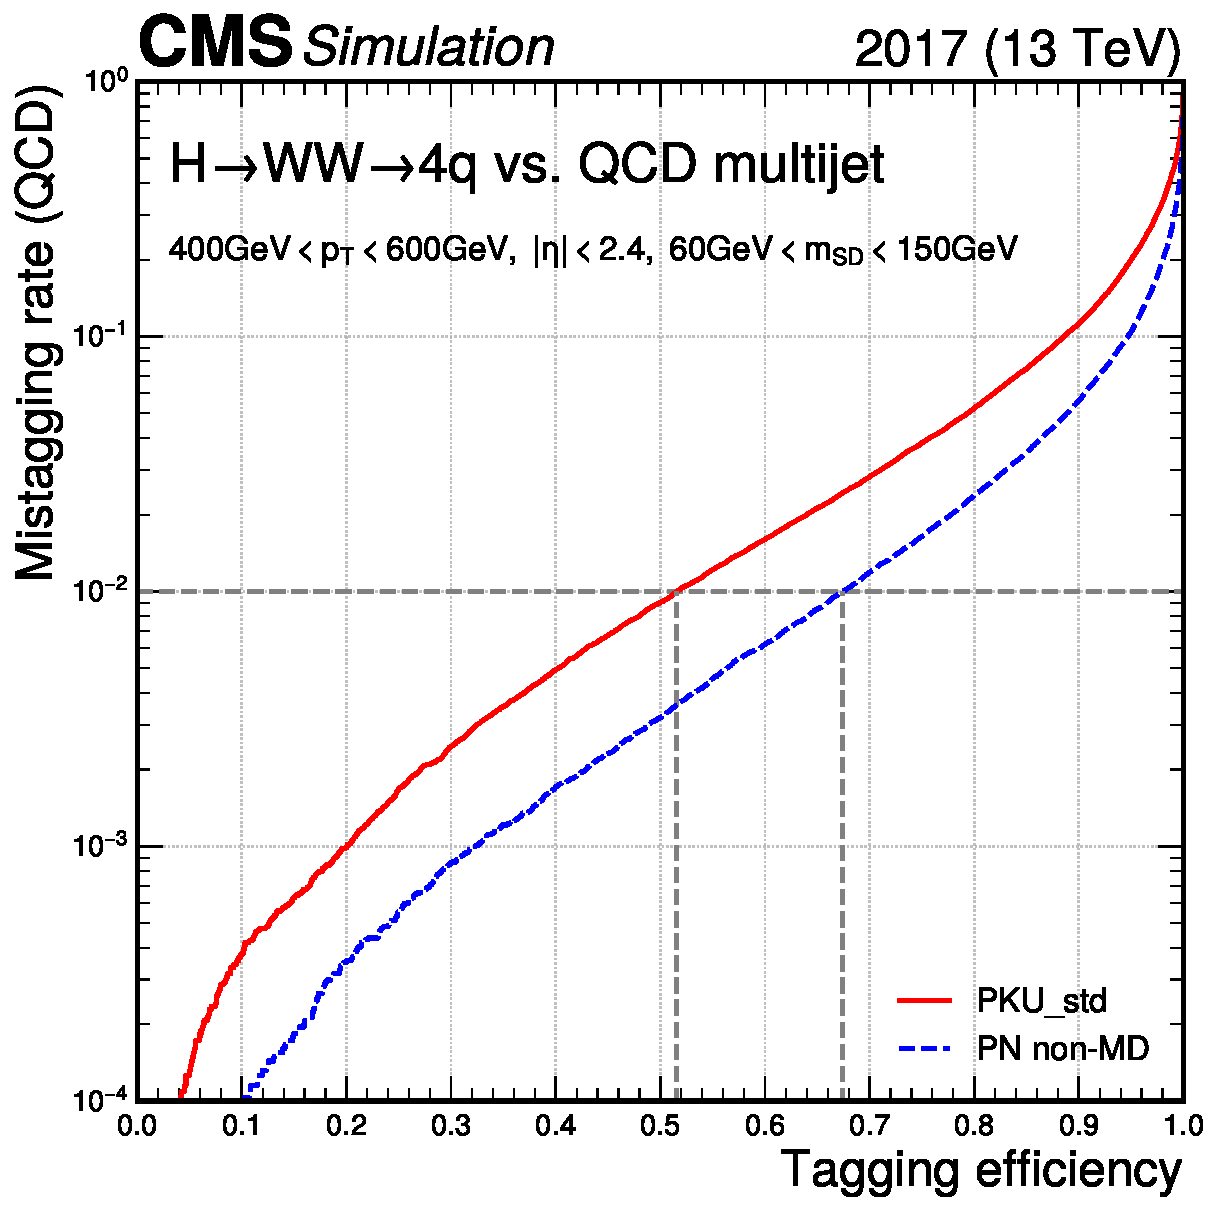
\includegraphics[height=12cm, width=12cm]{pictures/ROC_HWW_4q.pdf}
\end{figure}
这里PKU\_std是我们开发的质量去相关版本HWW多分类标记器,PN non-MD是原生ParticleNet的质量相关版本HWW4q单道标记器。在$Mistag\ rate=1\%$时,PKU\_std的$\text{Tagging efficiency}\approx52\%$,PN non-MD的Tagging efficiency$\approx68\%$。虽然PKU\_std比PN non-MD的效果要稍微差一些,但这正是质量去相关标记器的代价,换来的是被误鉴别的QCD本底没有接近信号峰的质量雕刻。如\textbf{图\ref{fig:5.3}}所示。

从\textbf{图\ref{fig:5.3}}可以看到,我们开发的质量去相关标记器PKU\_std的质量去相关效果非常好,在4q喷注的信号峰附近,QCD本底仍然保持了它原本的分布,没有形成类似4q喷注的质量峰分布,从而有利于我们在实验数据中提取4q信号。
而被PN non-MD误标记的QCD本底就有非常明显的质量雕刻现象,如\textbf{图\ref{fig:5.4}}所示。

\begin{figure}[H]
 \centering
 \caption{被PKU\_std误标记的QCD本底的$m_{SD}$分布}
 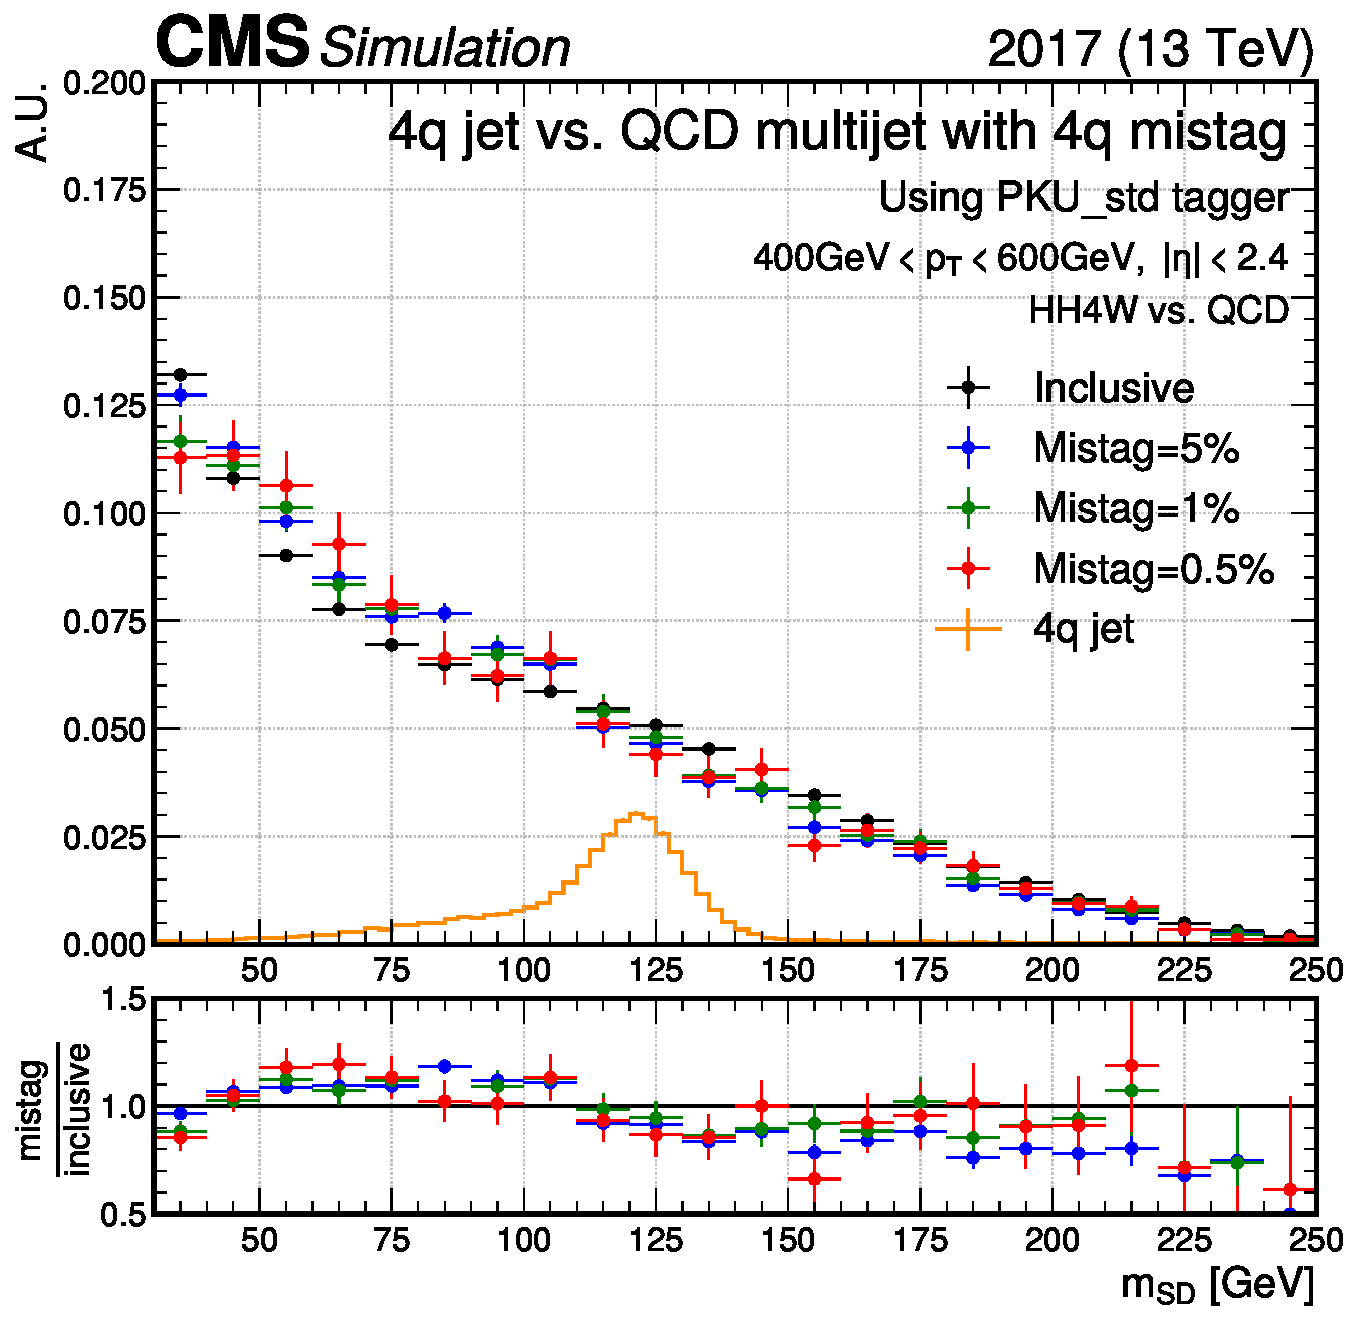
\includegraphics[height=9cm, width=9cm]{pictures/MD_PKU_std_4q.pdf}
 \label{fig:5.3}
\end{figure}

\begin{figure}[H]
 \centering
 \caption{被PN nonMD误标记的QCD本底的$m_{SD}$分布}
 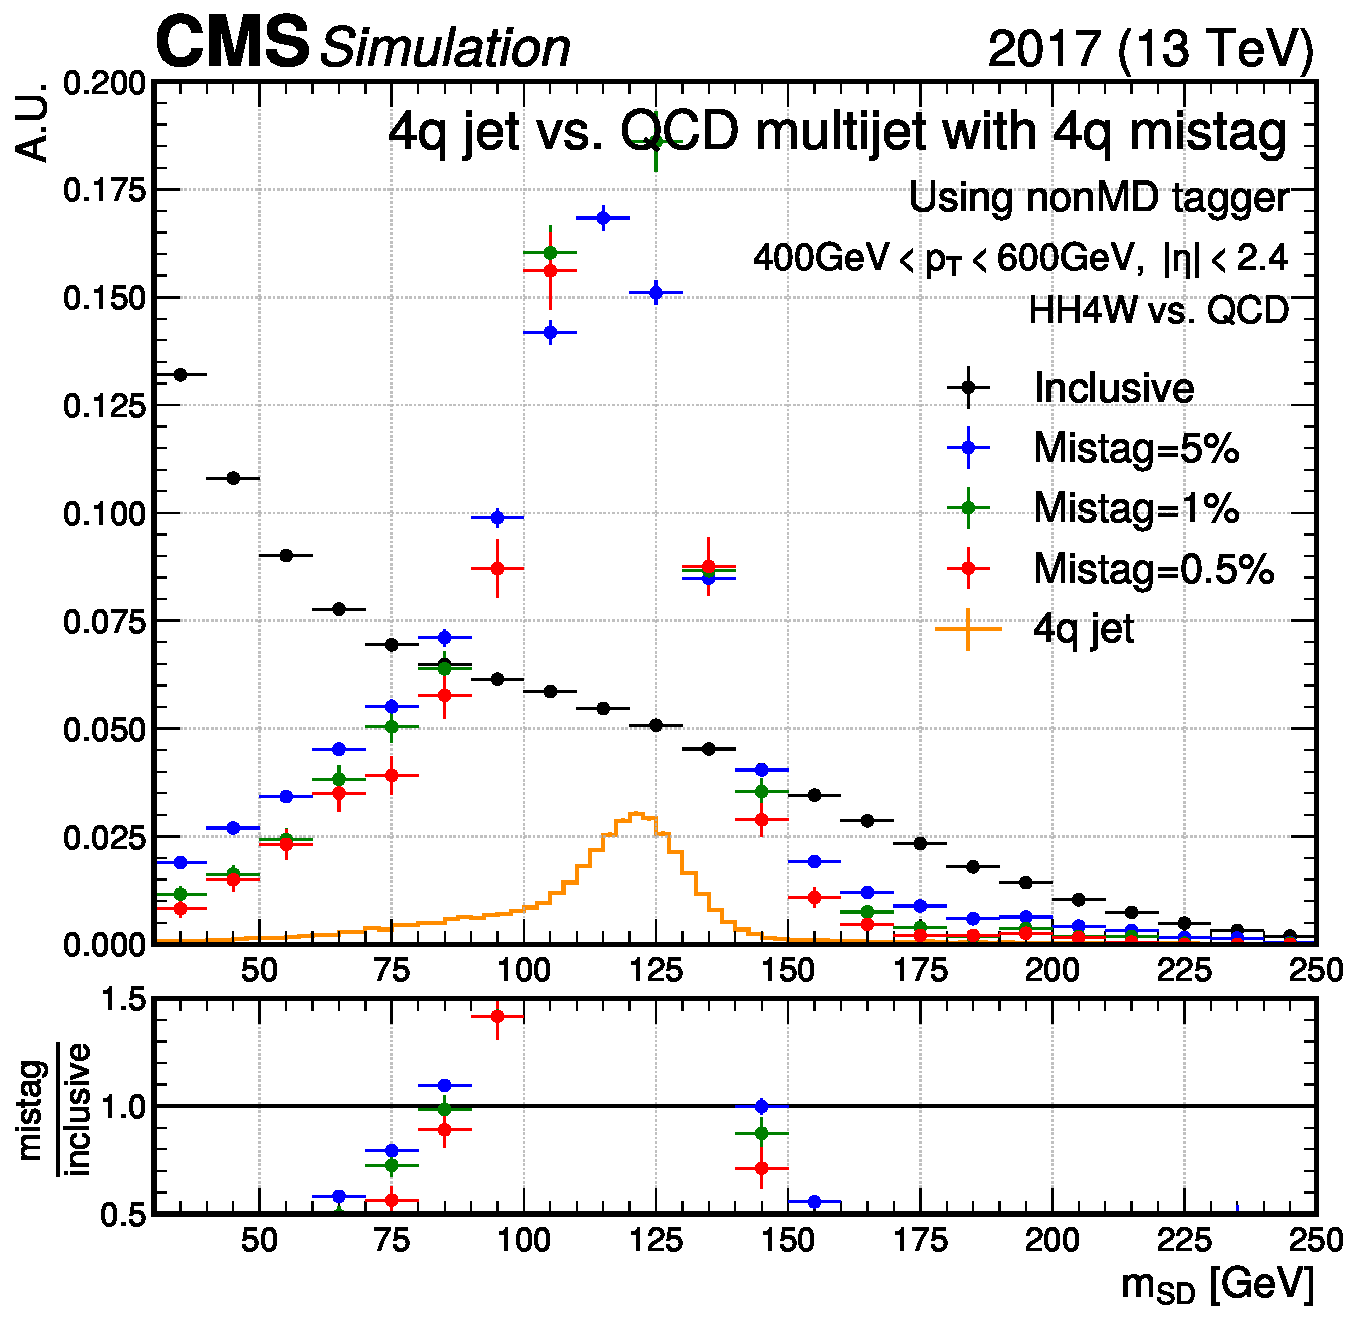
\includegraphics[height=9cm, width=9cm]{pictures/MD_nonMD_4q.pdf}
 \label{fig:5.4}
\end{figure}

比较以上两图我们可以看到,虽然PKU\_std比PN non-MD的效果要稍微差一些,但这正是质量去相关标记器的代价,以效率上20\%的损失换来了从无到有的质量去相关效果,极大地降低了分析难度。

除此之外,原有的PN non-MD只是$H\to W(2q)W(2q)$的单衰变道标记器,但我们开发的标记器是$H\to WW$的多衰变道标记器,所以在其他HWW衰变道上也有用武之地。
\begin{figure}[H]
 \centering
 \caption{我们开发的HWW标记器的对多个衰变道的标记性能}
 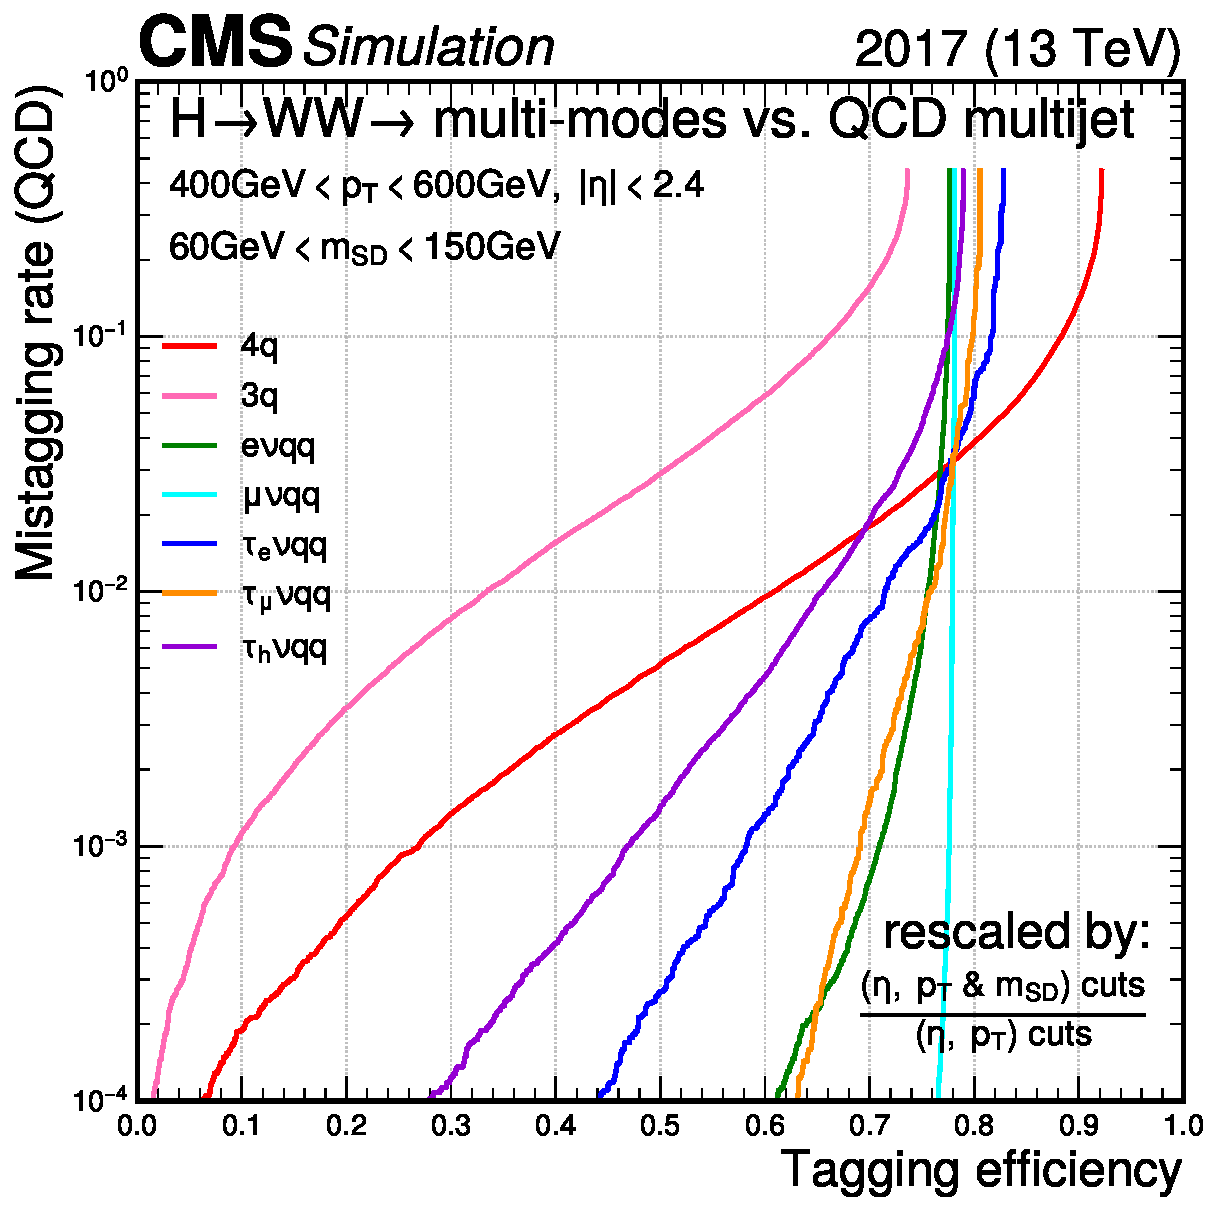
\includegraphics[height=11cm, width=11cm]{pictures/ROC_multi-modes_PKU_std.pdf}
 \label{fig:5.5}
\end{figure}
从这个图里我们可以看到,在Mistag rate=1\%时,除了3q末态(指HWW衰变到四个夸克但只有三个被重建在AK8喷注中)的标记效率只有33\%左右,其他几个道的标记啊效率都在60\%$\sim$80\%之间,更让我们对开发的标记器充满信心。
\section{在分析中的初步应用效果和前景}
我们目前已经将开发的标记器投入正式的CMS实验分析中使用,目前已经初步应用的分析场景为:\textbf{胶子聚合(ggF)产生大动量希格斯粒子,再到WW衰变的过程。}其费曼图如\textbf{图\ref{fig:2.4}左上}所示。

在此分析中,我们把我们开发的基于PaticleNet-MD的标记器和目前官方分析中针对AK8喷注常用的DeepAK8-MD标记器进行了比较。比较结果如下\textbf{图\ref{fig:5.6}}所示
\begin{figure}[H]
 \centering\label{fig:5.6}
 \caption{开发的PNet-MD标记器与DeepAK8标记器在$H\to WW\to4q$道的标记表现比较}
 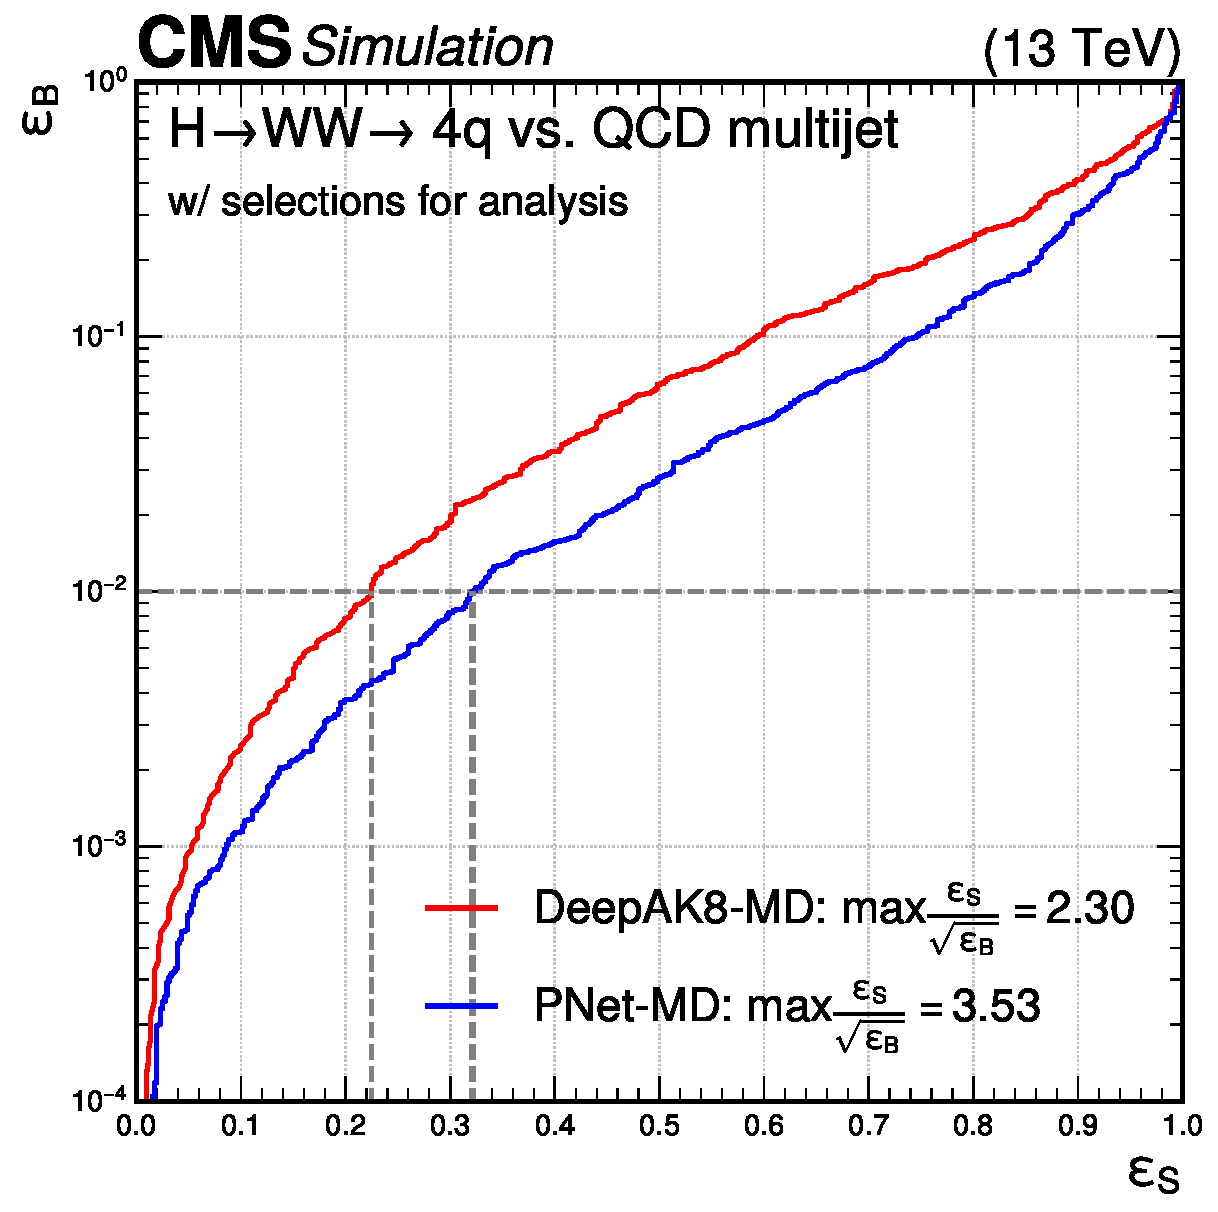
\includegraphics[height=10cm, width=10cm]{pictures/ana_roc_4q.pdf}
 \label{fig:5.6}
\end{figure}
\begin{comment}
\begin{figure}[H]
 \centering\label{fig:5.7}
 \caption{开发的PNet-MD标记器与DeepAK8标记器在$H\to WW\to\ell\nu qq$道的标记表现比较}
 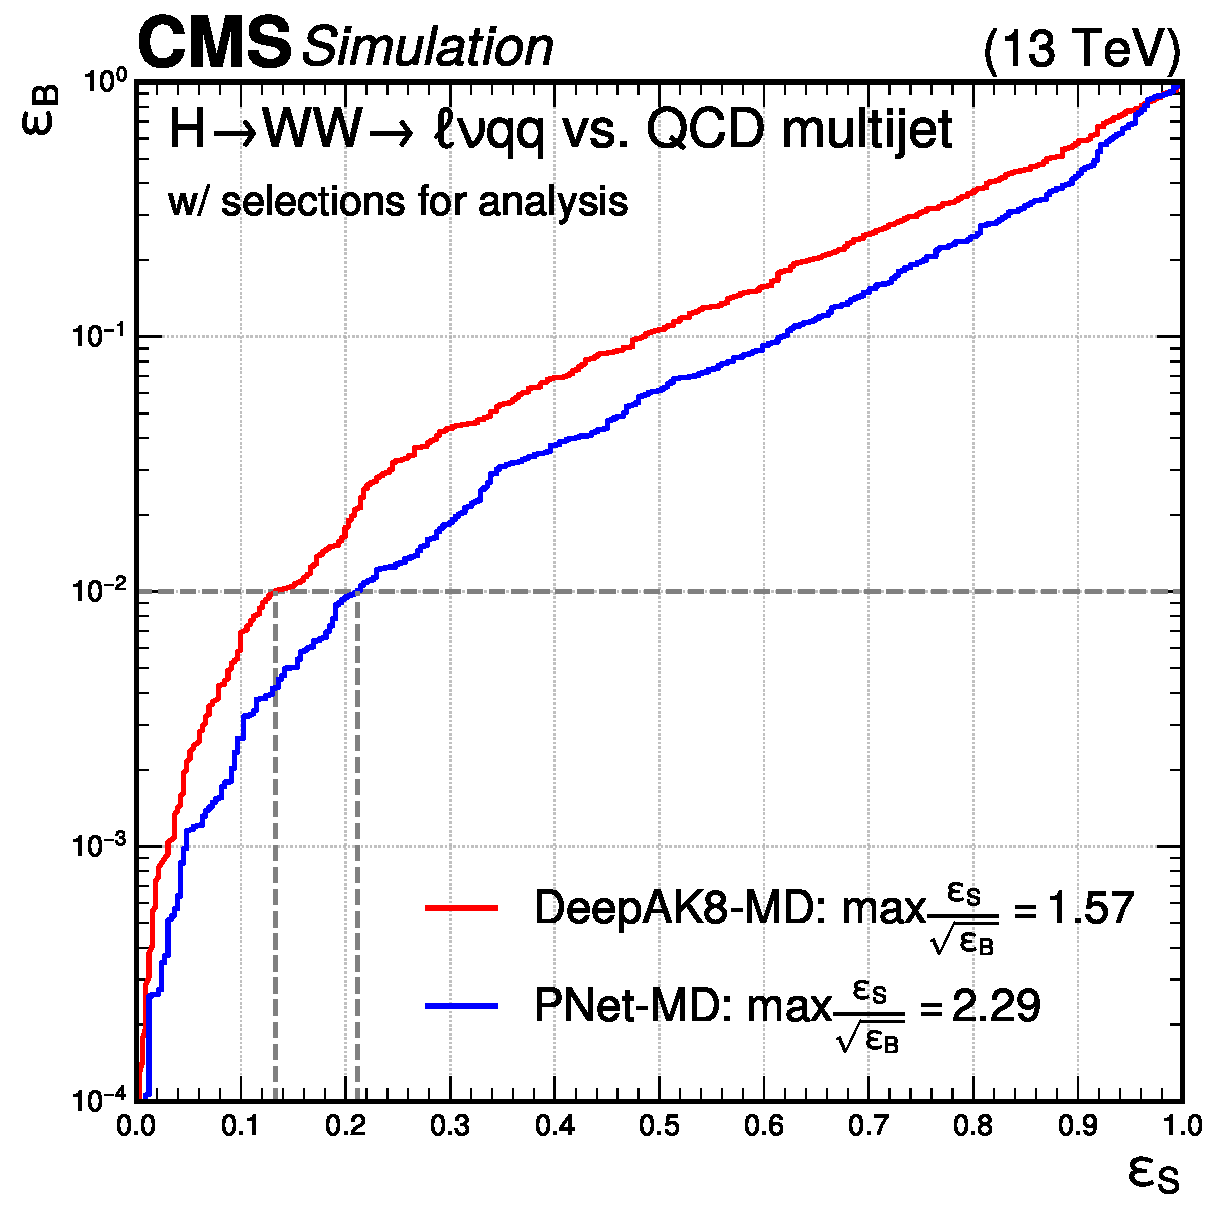
\includegraphics[height=10cm, width=10cm]{pictures/ana_roc_2q.pdf}
 \label{fig:5.7}
\end{figure}
\end{comment}
可以看到,我们开发的标记器与以往官方使用的标记器DeepAK8相比,在$g+g\to H\to WW$标记任务上有接近50\%的性能提升,并且随着日后更多的研究和采用更大规模网络模型,标记器的表现还有更大的提升空间。

除此之外,我们的$H\to WW$标记器还有更多值得期待的分析应用场景,包括:
\begin{enumerate}[$\bullet$]
    \item 标记VBF、WH等大动量希格斯粒子产生过程:以研究大$p_T$希格斯粒子的物理性质和间接搜寻高能标的超标准模型物理迹象。
    \item $HH\to WWWW$和$HH\to bbWW$过程:可以在这样的过程中测量希格斯粒子自耦合强度,同时搜寻双希格斯共振态。
    \item 对暗物质的搜寻:因为我们开发的标记器的输入不包括中微子信息,所以设计场景中存在消失的横向动量(MET),可以借此搜寻$H+\text{MET (Dark Matter)}\to WW$的暗物质过程。
\end{enumerate}